% Short paper (candidate: a 4-page IEEE short/workshop track, e.g. an MSR or ICSME short paper). Venue not final.
% Tool + measurement study in one paper. Every number comes from ../generated/*.tex, built by
% ../scripts/make_paper_numbers.py from research/experiments/benchmark/results (see ../CLAIMS.md).
\documentclass[10pt,conference]{IEEEtran}
\usepackage[T1]{fontenc}
\usepackage{booktabs,graphicx,url,amsmath,xspace}
\usepackage[hidelinks]{hyperref}
% generated by scripts/make_paper_numbers.py
\newcommand{\nCorpus}{54{,}058\xspace}
\newcommand{\nAnchored}{51{,}697\xspace}
\newcommand{\nUnres}{2{,}361\xspace}
\newcommand{\pctUnres}{4.4\xspace}
\newcommand{\pctReach}{56.6\xspace}
\newcommand{\ciReach}{[56.2, 57.1]\xspace}
\newcommand{\ciReachRepo}{[53.9, 59.3]\xspace}
\newcommand{\pctReachHigh}{44.8\xspace}
\newcommand{\ciReachHigh}{[44.4, 45.3]\xspace}
\newcommand{\meanReach}{18.8\xspace}
\newcommand{\ciMeanReach}{[18.6, 19.1]\xspace}
\newcommand{\medianReach}{1.3\xspace}
\newcommand{\nRepos}{8{,}548\xspace}
\newcommand{\nTyped}{2{,}630\xspace}
\newcommand{\catUnrel}{42.9\xspace}
\newcommand{\catDocs}{22.6\xspace}
\newcommand{\catTests}{15.7\xspace}
\newcommand{\catFmt}{12.6\xspace}
\newcommand{\catDeps}{7.8\xspace}
\newcommand{\catCI}{5.8\xspace}
\newcommand{\reachClaude}{52.6\xspace}
\newcommand{\stdClaude}{55.9\xspace}
\newcommand{\filesClaude}{4\xspace}
\newcommand{\bigClaude}{16.8\xspace}
\newcommand{\reachCopilot}{82.3\xspace}
\newcommand{\stdCopilot}{62.9\xspace}
\newcommand{\filesCopilot}{15\xspace}
\newcommand{\bigCopilot}{46.3\xspace}
\newcommand{\reachCodex}{56.4\xspace}
\newcommand{\stdCodex}{58.3\xspace}
\newcommand{\filesCodex}{4\xspace}
\newcommand{\bigCodex}{16.2\xspace}
\newcommand{\reachCursor}{67.6\xspace}
\newcommand{\stdCursor}{66.5\xspace}
\newcommand{\filesCursor}{5\xspace}
\newcommand{\bigCursor}{19.3\xspace}
\newcommand{\reachDevin}{49.9\xspace}
\newcommand{\stdDevin}{57.0\xspace}
\newcommand{\filesDevin}{3\xspace}
\newcommand{\bigDevin}{12.6\xspace}
\newcommand{\reachJules}{40.4\xspace}
\newcommand{\stdJules}{57.9\xspace}
\newcommand{\filesJules}{2\xspace}
\newcommand{\bigJules}{11.0\xspace}
\newcommand{\missCopilot}{1.2\xspace}
\newcommand{\missAll}{1.3\xspace}
\newcommand{\noncodeCopilot}{11.7\xspace}
\newcommand{\noncodeAll}{19.5\xspace}
\newcommand{\readmeCopilot}{11.4\xspace}
\newcommand{\readmeOther}{6.6\xspace}
\newcommand{\instrCopilot}{5.0\xspace}
\newcommand{\instrOther}{0.1\xspace}
\newcommand{\pkgCopilot}{7.9\xspace}
\newcommand{\pkgOther}{3.3\xspace}
\newcommand{\mergedReach}{57.9\xspace}
\newcommand{\unmergedReach}{54.1\xspace}
\newcommand{\mergeRaw}{+3.8\xspace}
\newcommand{\mergeStd}{-0.5\xspace}
\newcommand{\ciMergeStd}{[-4.5, 2.9]\xspace}
\newcommand{\taskFeat}{84.8\xspace}
\newcommand{\taskNFeat}{1{,}087\xspace}
\newcommand{\taskFix}{63.7\xspace}
\newcommand{\taskNFix}{1{,}022\xspace}
\newcommand{\taskRefactor}{82.3\xspace}
\newcommand{\taskNRefactor}{169\xspace}
\newcommand{\taskDocsTask}{66.2\xspace}
\newcommand{\taskNDocsTask}{162\xspace}
\newcommand{\unresDocsTask}{19.8\xspace}
\newcommand{\nPai}{3{,}087\xspace}
\newcommand{\nPaiSC}{455\xspace}
\newcommand{\nPaiUnres}{21\xspace}
\newcommand{\nPaiBench}{500\xspace}
\newcommand{\nPaiGym}{2{,}287\xspace}
\newcommand{\nPaiML}{300\xspace}
\newcommand{\aucFence}{0.577\xspace}
\newcommand{\ciAucFence}{[0.554, 0.601]\xspace}
\newcommand{\aucSize}{0.757\xspace}
\newcommand{\ciAucSize}{[0.733, 0.779]\xspace}
\newcommand{\aucFiles}{0.673\xspace}
\newcommand{\aucTfidf}{0.577\xspace}
\newcommand{\aucDirs}{0.510\xspace}
\newcommand{\paiBudget}{769\xspace}
\newcommand{\precFence}{23.0\xspace}
\newcommand{\recFence}{38.9\xspace}
\newcommand{\precSize}{31.9\xspace}
\newcommand{\recSize}{53.8\xspace}
\newcommand{\cvSize}{0.756\xspace}
\newcommand{\cvSizeFence}{0.757\xspace}
\newcommand{\cvDelta}{+0.002\xspace}
\newcommand{\ciCvDelta}{[-0.001, +0.005]\xspace}
\newcommand{\tercSmall}{0.529\xspace}
\newcommand{\tercMid}{0.550\xspace}
\newcommand{\tercLarge}{0.517\xspace}
\newcommand{\latMedian}{3.3\xspace}
\newcommand{\latPninety}{23.6\xspace}
\newcommand{\latPnn}{126\xspace}
\newcommand{\latN}{2{,}000\xspace}
\newcommand{\goldPRs}{300\xspace}
\newcommand{\goldFiles}{1{,}471\xspace}
\newcommand{\goldUnres}{19\xspace}
\newcommand{\goldPerAgent}{50\xspace}
\newcommand{\rhoSize}{0.34\xspace}
\newcommand{\rhoFiles}{0.50\xspace}

\begin{document}
\title{Beyond the Issue: Flagging and Measuring\\What Coding-Agent Pull Requests Change Unasked}
\author{\IEEEauthorblockN{Harshul Jain}\IEEEauthorblockA{Independent Researcher}}
\maketitle

\begin{abstract}\normalfont
Reviewers of pull requests (PRs) opened by coding agents often compare the linked issue with the changed files by hand, looking for ``helpful'' extras nobody asked for. We present Fence, a deterministic, CPU-only checker and GitHub Action that flags each changed file or formatting-only hunk that nothing in the issue points to, and says why. We run it on \nCorpus{} agent PRs from the public AIDev dataset. By Fence's flags, \pctReach\% of the PRs it could anchor to their issue change at least one such part, and on average \meanReach\% of a PR's changed lines are outside the issue. Agents range from \reachJules\% to \reachCopilot\%, but most of the gap follows PR size: at the same file-count mix Copilot drops to \stdCopilot\%. Our headline result is negative. On \nPai{} human scope-creep labels from PAIChecker, plain PR size ranks scope creep better than Fence (AUROC \aucSize{} vs \aucFence), and adding Fence to size does not help (\cvDelta{} \ciCvDelta). Fence's precision is not yet measured: a \goldPRs-PR gold sheet is ready for human labels. All rates here are tool output, not verified prevalence.
\end{abstract}

\section{Introduction}
Coding agents now open hundreds of thousands of PRs on GitHub~\cite{li2026aidev}. A common complaint is that they do more than they were asked: they reformat files, bump dependencies, edit CI or rewrite code the issue never mentioned. Such extras matter. In a study of 33{,}580 agent PRs, unintended side effects (22.33\%) and overengineering (22.13\%) were more common causes of later reverts than functional bugs (17.71\%)~\cite{oukhay2026revert}. Tangled changes are known to cost reviewers and to bias mining studies~\cite{herzig2013tangled}.

Prior work compared the PR \emph{description} with the code~\cite{gong2026prmci}, or used LLMs to judge whether a whole PR matches its issue, on small sets of human PRs~\cite{isik2025forge,altunhan2026finetune} and on SWE-bench-style benchmarks~\cite{wang2026paichecker}. Agent out-of-scope actions were also measured in sandboxes~\cite{qu2026overeager,trong2026swemisbehavior}. Industry has started on the same problem. Meta's ARCTIC detects \emph{drift}, including unrequested changes, by comparing an LLM back-translation of the diff with the intent inferred from the agent's conversation logs~\cite{maddila2026arctic}. Microsoft researchers replay agent trajectories and rerun tests to decide which edits in benchmark patches are needed~\cite{goel2026overedit}. Both need an LLM, trajectories or tests, and evaluate on internal or benchmark data. What is still missing is a cheap check that uses only the linked issue and the diff, explains each flag, and is measured on public agent PRs at scale.

We contribute: (1) Fence, an open-source checker and GitHub Action that explains each flag (\S\ref{sec:fence}); (2) scope-reach rates on \nCorpus{} agent PRs from \nRepos{} repositories, by agent, task type and kind of extra, showing that PR size explains most of the difference between agents; and (3) a check against independent human labels, where PR size beats Fence. We state plainly what we have not measured: Fence's precision on agent PRs.

\section{Fence}\label{sec:fence}
\textbf{Reading the issue.} Fence~ extracts the paths, directories, code names (\texttt{camelCase}, \texttt{snake\_case}, dotted names, backticked spans) and distinctive words in the issue title and body, dropping common English and issue-template words.

\textbf{Checking each part.} The diff is split into files, and formatting-only hunks are found by comparing tokens without whitespace. A file is in scope if the issue names it, its directory or its stem; if its changed code touches a name from the issue; if its path and changed names share enough issue terms; or if it is a companion of an in-scope file (its test, or a file that wires in an in-scope module). Every other part is flagged with a reason and a category: unrelated code (``edits a code file that no path, name or term in the issue points to'', naming the changed symbols), docs, tests, CI, dependencies, or formatting-only hunks. CI and dependency edits are high severity unless the issue mentions them; formatting is low. If the issue names nothing concrete, Fence reports the PR as \emph{scope unresolvable} and flags only CI, dependency and formatting parts instead of guessing. \emph{Scope reach} is the share of changed lines in flagged parts.

\textbf{Using it.} \texttt{pip install rd0-fence} provides a \texttt{fence} command that reads an issue and a diff, or fetches both from GitHub. The composite Action finds the linked issue in the same repository only and keeps a single comment up to date (Fig.~\ref{fig:comment}). Fence is pure Python with no runtime dependencies and needs no API key, so no code leaves the CI runner. On \latN{} random corpus PRs it takes a median of \latMedian\,ms per PR in one CPU process (90th percentile \latPninety\,ms, 99th \latPnn\,ms).

\begin{figure}[t]\centering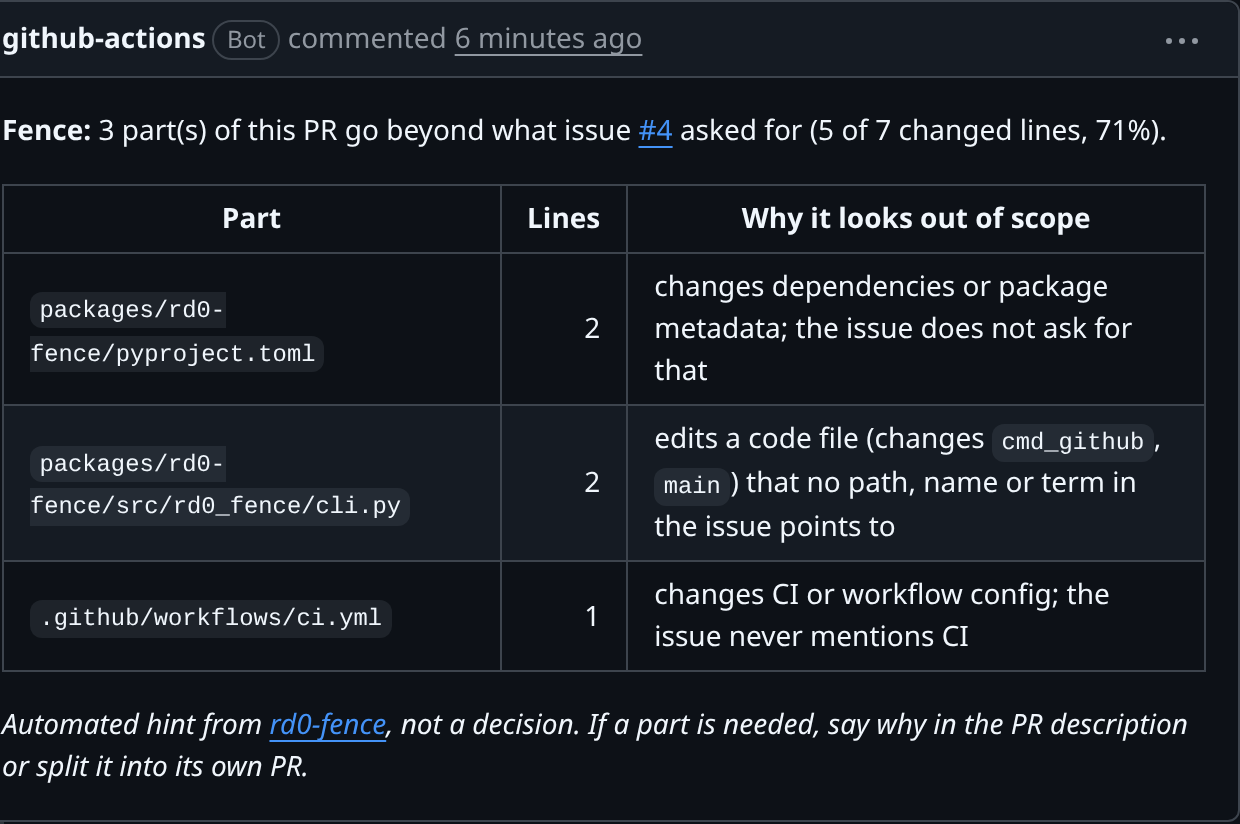
\includegraphics[width=\columnwidth]{fig_action_comment.png}
\caption{Fence's comment on a demo PR whose issue asked only for a documentation fix: each extra file, with a reason.}\label{fig:comment}\end{figure}

\section{Study Design}
\textbf{Data.} AIDev v5~\cite{li2026aidev} (CC BY 4.0) lists agent PRs with their linked issues and per-commit file patches. We keep PRs whose linked issue has usable text and whose changed files carry patches for at least 90\% of file rows: \nCorpus{} PRs. Task types come from AIDev-full's labels and cover \nTyped{} of them. The \nUnres{} scope-unresolvable PRs (\pctUnres\%) are excluded from rates.

\textbf{Statistics.} A PR \emph{reaches} if Fence flags any part. Rates have Wilson 95\% intervals, means have bootstrap intervals, and the overall rate also has a repository-clustered bootstrap interval.

\textbf{External labels and baselines.} PAIChecker~\cite{wang2026paichecker} released human labels for issue/patch pairs in SWE-bench~\cite{jimenez2024swebench}, SWE-Gym~\cite{pan2025swegym} and SWE-bench Multilingual; one label is scope creep. We score \nPai{} labelled instances (\nPaiSC{} scope creep) and compare Fence with four baselines: PR size in changed lines, file count, top-level directories and TF-IDF distance between issue and diff.

\section{Results}
\subsection*{RQ1: How often do agent PRs reach beyond their issue?}
Fence flags at least one part in \pctReach\% \ciReach{} of anchored PRs (repository-clustered \ciReachRepo), and a high-severity part in \pctReachHigh\%. The distribution is skewed: mean reach is \meanReach\%, median \medianReach\%. Table~\ref{tab:agents} breaks this down by agent. The most common extras are unrelated code (\catUnrel\% of PRs), docs (\catDocs\%), tests (\catTests\%), formatting-only hunks (\catFmt\%), dependencies (\catDeps\%) and CI (\catCI\%).

\begin{table}[t]\centering\caption{Fence's flags by agent (tool output, not verified). Unres.: scope unresolvable. Any / High: PRs with any / high-severity flag. Mean: share of changed lines flagged. Std.: any-flag rate re-weighted to the overall file-count mix.}\label{tab:agents}
\footnotesize\setlength{\tabcolsep}{2.6pt}\begin{tabular}{@{}lrrrrrrr@{}}\toprule
Agent & PRs & Unres.\,\% & Any\,\% & High\,\% & Mean\,\% & Files & Std.\,\%\\\midrule
Claude Code & 40{,}259 & 4.3 & 52.6 & 41.6 & 17.6 & 4 & 55.9\\
Copilot & 6{,}549 & 5.0 & 82.3 & 70.0 & 28.1 & 15 & 62.9\\
Codex & 5{,}258 & 3.9 & 56.4 & 38.9 & 16.6 & 4 & 58.3\\
Cursor & 786 & 4.6 & 67.6 & 54.0 & 23.9 & 5 & 66.5\\
Devin & 961 & 5.3 & 49.9 & 37.7 & 16.6 & 3 & 57.0\\
Jules & 245 & 6.9 & 40.4 & 35.1 & 16.3 & 2 & 57.9\\
\midrule
All & 54{,}058 & 4.4 & 56.6 & 44.8 & 18.8 & 5 & 56.6\\
\bottomrule

\end{tabular}\end{table}

\subsection*{RQ2: Which tasks reach furthest?}
Among the \nTyped{} PRs with a task type (Table~\ref{tab:tasks}), features (\taskFeat\%) and refactorings (\taskRefactor\%) reach more often than fixes (\taskFix\%). Documentation tasks have the most vague issues (\unresDocsTask\% unresolvable). These subsets are small and their intervals wide.

\begin{table}[t]\centering\caption{Fence's flags by task type (AIDev-full labels; types with at least 10 PRs).}\label{tab:tasks}
\footnotesize\begin{tabular}{@{}lrrrr@{}}\toprule
Task & PRs & Unres.\,\% & Any flag\,\% [95\% CI] & Mean reach\,\%\\\midrule
feat & 1{,}087 & 3.4 & 84.8 [82, 87] & 29.1\\
fix & 1{,}022 & 3.4 & 63.7 [61, 67] & 23.8\\
refactor & 169 & 3.0 & 82.3 [76, 87] & 27.8\\
docs & 162 & 19.8 & 66.2 [58, 74] & 36.4\\
test & 60 & 1.7 & 74.6 [62, 84] & 32.6\\
chore & 62 & 12.9 & 53.7 [41, 66] & 21.9\\
build & 41 & 12.2 & 69.4 [53, 82] & 38.1\\
\bottomrule

\end{tabular}\end{table}

\subsection*{RQ3: What explains the differences?}
Mostly PR size. Bigger PRs give Fence more parts to flag, and its reach correlates with file count (Spearman $\rho=\rhoFiles$). Copilot's PRs have a median of \filesCopilot{} files against \filesClaude{} for Claude Code, and \bigCopilot\% change more than 16 files (Claude Code: \bigClaude\%). Re-weighting each agent to the corpus file-count mix shrinks the spread from \reachJules--\reachCopilot\% to \stdClaude--\stdCursor\% (Table~\ref{tab:agents}, Fig.~\ref{fig:bins}). Missing patches do not explain it (\missCopilot\% of Copilot file rows, \missAll\% overall). What remains is partly template files: Copilot PRs edit \texttt{README.md} (\readmeCopilot\% vs \readmeOther\% for other agents), \texttt{package.json} (\pkgCopilot\% vs \pkgOther\%) and its own \texttt{copilot-instructions.md} (\instrCopilot\% vs \instrOther\%) without being asked.

The same caution applies to outcomes. Merged PRs are flagged slightly more often than unmerged ones (\mergedReach\% vs \unmergedReach\%, \mergeRaw{} points), but at the same file-count mix the difference is \mergeStd{} points \ciMergeStd. We find no evidence that Fence's flags predict merging once size is held fixed.

\begin{figure}[t]\centering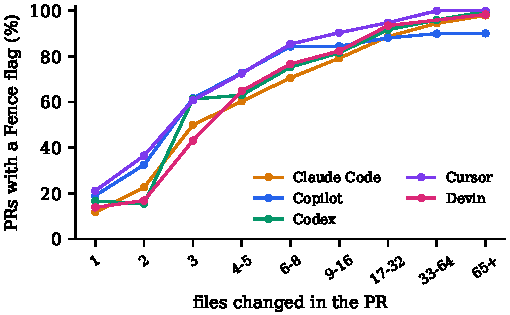
\includegraphics[width=\columnwidth]{../generated/fig_bins.pdf}
\caption{Share of PRs with a Fence flag by number of changed files (bins with fewer than 30 PRs omitted). Agents differ far less within a size bin than overall.}\label{fig:bins}\end{figure}

\subsection*{RQ4: Do Fence's flags agree with human scope-creep labels?}
No better than PR size (Table~\ref{tab:pai}, Fig.~\ref{fig:auroc}). On PAIChecker's labels, PR size reaches AUROC \aucSize{} \ciAucSize{} and Fence's reach \aucFence{} \ciAucFence. Flagging the same \paiBudget{} instances that Fence flags, PR size has \precSize\% precision and \recSize\% recall, Fence \precFence\% and \recFence\%. In 5-fold cross-validated logistic regression, adding Fence to size changes AUROC from \cvSize{} to \cvSizeFence{} (paired bootstrap gain \cvDelta{} \ciCvDelta), and within PR-size terciles Fence's AUROC is \tercSmall, \tercMid{} and \tercLarge. Two differences limit the comparison: the labels are per PR on human-written gold patches, not agent PRs, and PAIChecker's scope creep includes over-reach inside files the issue does name, which file-level rules cannot see. Still, a large PR remains the better single warning sign; Fence's possible value is in saying \emph{which} part to look at and \emph{why}, which these labels cannot test.

\begin{table}[t]\centering\caption{AUROC against PAIChecker's human scope-creep labels (\nPai{} instances, bootstrap 95\% CI), overall and per source set (SWE-bench / SWE-Gym / Multilingual).}\label{tab:pai}
\footnotesize\setlength{\tabcolsep}{2.5pt}\begin{tabular}{@{}lccc c@{}}\toprule
Score & All & Bench & Gym & ML\\\midrule
PR size (changed lines) & 0.757 [0.733, 0.779] & 0.75 & 0.74 & 0.75\\
File count & 0.673 [0.646, 0.698] & 0.64 & 0.65 & 0.70\\
\textbf{Fence reach} & 0.577 [0.554, 0.601] & 0.54 & 0.56 & 0.66\\
TF-IDF issue/diff distance & 0.577 [0.550, 0.603] & 0.69 & 0.56 & 0.52\\
Top-level directories & 0.510 [0.489, 0.532] & 0.52 & 0.48 & 0.59\\
\bottomrule

\end{tabular}\end{table}

\begin{figure}[t]\centering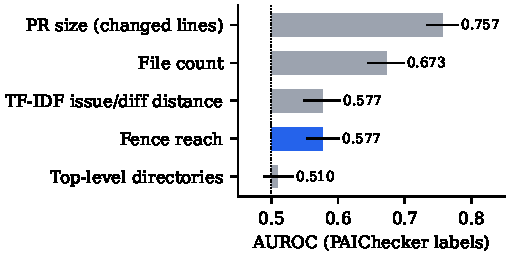
\includegraphics[width=\columnwidth]{../generated/fig_auroc.pdf}
\caption{PR size ranks PAIChecker's scope-creep labels better than Fence.}\label{fig:auroc}\end{figure}

\subsection*{Gold sheet: Fence's precision (not yet measured)}
To measure whether Fence's part-level flags are right on agent PRs, we drew a gold sheet of \goldPRs{} PRs (\goldPerAgent{} per agent, \goldFiles{} files, \goldUnres{} that Fence calls unresolvable) and built a labeling app in which annotators mark each file in scope, out of scope or \emph{scope unresolvable}. No human has labelled it yet. Table~\ref{tab:gold} is a placeholder: it holds no numbers.

\begin{table}[t]\centering\caption{PLACEHOLDER. Gold-sheet results, to be filled after two annotators label the \goldPRs{} PRs. No value has been measured.}\label{tab:gold}
\footnotesize\begin{tabular}{@{}ll@{}}\toprule
Measure (file level) & Value\\\midrule
Precision of Fence's flags & not yet measured\\
Recall of human out-of-scope files & not yet measured\\
Inter-annotator agreement (Cohen's $\kappa$) & not yet measured\\
PRs humans call scope unresolvable & not yet measured\\
\bottomrule\end{tabular}\end{table}

\section{Threats to Validity}
\emph{Construct.} Every rate is Fence's output. Fence can be wrong in both directions: it flags support edits a reviewer would accept (an import, a fixture), and it misses over-reach inside in-scope files. Some extras are welcome: a maintainer may ask for them in comments rather than in the issue. \emph{Internal.} AIDev stores one patch per commit and file, so lines rewritten across commits can be counted twice. \emph{External.} Copilot PRs often lack patches and are under-represented, and the task-type subset is small.

\section{Related Work}
PR-MCI~\cite{gong2026prmci} measured disagreement between an agent PR's description and its code, not its issue. I\c{s}{\i}k et al.~\cite{isik2025forge} and Altunhan et al.~\cite{altunhan2026finetune} used LLMs to classify issue/PR pairs as exact, missing or tangled. PAIChecker~\cite{wang2026paichecker} found misaligned issue/patch pairs in SWE-bench-like benchmarks. Overeager agents~\cite{qu2026overeager}, SWE-Misbehavior~\cite{trong2026swemisbehavior} and Refactoring Runaway~\cite{tian2026runaway} study out-of-scope agent behaviour in controlled settings. Closest to our setting, ARCTIC~\cite{maddila2026arctic} scores drift between inferred intent and the diff with an LLM inside Meta, and Goel et al.~\cite{goel2026overedit} find that most extra edits in agent patches on SWE-bench Verified are tests (61\%) and documentation (13\%), and argue that patch size alone cannot show whether extra edits are needed. In real agent sessions, Tang et al.~\cite{tang2026fail} classify 10.20\% of misalignment episodes as self-initiated overreach; SNARE~\cite{qu2026snare} and ParanoiaEval~\cite{luo2026paranoia} elicit overeager and unnecessary defensive behaviour, and Ehsani et al.~\cite{ehsani2026fail} study why agent PRs fail. Unlike these, Fence uses only the linked issue and the diff, works on individual files and hunks, needs no LLM, trajectory or tests, and is evaluated on public agent PRs.

\section{Conclusion}
By a deterministic checker's flags, more than half of agent PRs with a linked issue change something the issue does not point to, but agent differences mostly follow PR size, and on independent human labels PR size is the better signal. The next step is to label the gold sheet and report Fence's precision. Fence, its Action, per-PR scores, the gold sheet and the labeling app are at \url{https://github.com/ReviewDebtZero/rd0-fence}; a demo is at \url{https://rd0-fence.netlify.app}.

\bibliographystyle{IEEEtran}
\bibliography{../refs}
\end{document}
